\documentclass[12pt]{article}
\usepackage[numbers]{natbib}
\usepackage{graphicx}
\usepackage{amsmath}
\usepackage{hyperref}
\usepackage{geometry}
\usepackage{subcaption}
\usepackage{float}
\geometry{a4paper, margin=1in}

\title{\textbf{Subsurface Features of Lunar Pits} \\ A Contemporary Survey}
\author{Michal Glos (213396)}
\date{December 2024}

\begin{document}

\maketitle

\begin{abstract}
Lunar pits, revealed through high-resolution orbital imagery, are compelling geological features that provide access to the Moon's subsurface. These structures offer critical insights into ancient volcanic activity, expose the stratigraphy of the lunar crust, and present opportunities for future exploration. This survey consolidates current understanding of their morphology, formation mechanisms, thermal properties, and spatial distribution. By leveraging data from key missions such as the Lunar Reconnaissance Orbiter (LRO) and SELENE, this work highlights the significant discoveries made regarding these features. Lunar pits are emerging as pivotal elements in lunar science, with the potential to reshape exploration strategies and resource utilization in the years ahead.
\end{abstract}

\graphicspath{{img/ch1}}

\section{Introduction}
Lunar pits are remarkable geological formations that differ significantly from impact craters and volcanic vents. Characterized by steep vertical walls, these features often provide direct access to subsurface voids, such as collapsed lava tubes, tectonic cavities, or impact-induced hollows \cite{lunar-pit-distribution, lunar-pits-entrances-to-caves, new-wagner}. Their discovery, largely enabled by high-resolution imagery from the Lunar Reconnaissance Orbiter (LRO) Narrow Angle Camera (NAC) and the SELENE spacecraft, has revolutionized our understanding of the Moon's crustal architecture, composition, and dynamic history. For example, GRAIL and SELENE data reveal gravity anomalies and radar echoes consistent with intact lava tubes beneath some pits, such as the Marius Hills region \cite{GRAIL, cavities-selene-lavatubes, grails-gradients-mariushills}.

Beyond their geological intrigue, lunar pits hold practical importance for future exploration. These natural formations offer stable thermal environments, shielding from cosmic radiation, and protection from micrometeoroid impacts, making them attractive candidates for human habitation, resource storage, and scientific research stations \cite{bases-feng, newer-thermal, radar-observations-lava-tubes}. Notably, the Mare Tranquillitatis pit (see Fig.~\ref{fig:image1}), a vertical shaft with visible stratigraphic layers, exemplifies the potential of such features to provide insights into lunar geology and serve as access points to extensive cave systems. Radar imaging has further confirmed a subsurface cave conduit beneath the Mare Tranquillitatis pit, supporting its suitability as a target for human exploration \cite{Carrer2024, grails-gradients-mariushills}.

Lunar pits expose ancient stratigraphic layers, revealing records of volcanic flows and crustal evolution. Observations from missions such as SELENE and LRO confirm that these features likely formed through roof collapses above voids, such as lava tubes, highlighting their volcanic origin. For example, the Mare Tranquillitatis pit has been modeled to result from impacts triggering collapses in lava tube roofs, a process corroborated by gravitational anomalies and radar data \cite{lunar-pits-numerical-modelling, radar-observations-lava-tubes, cavities-selene-lavatubes}. The internal layering visible in pits, such as those in Mare Tranquillitatis and Marius Hills, provides key data on successive volcanic episodes, supporting broader studies on lunar surface evolution \cite{sublunear-lava, newer-thermal, bases-feng}.

\begin{figure}[h!]
    \centering
    \begin{subfigure}[c]{0.59\linewidth}
        \centering
        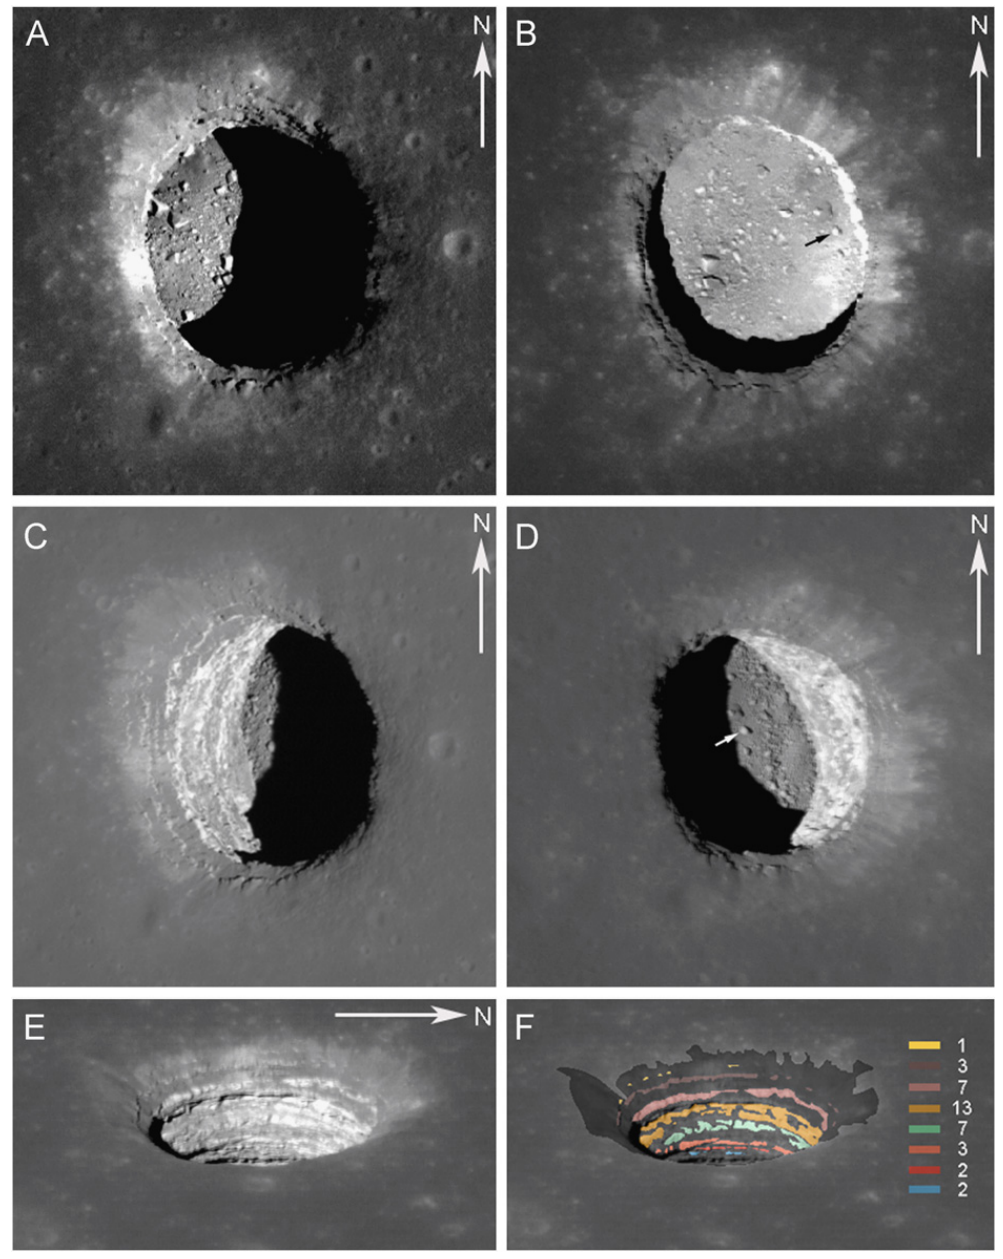
\includegraphics[width=0.9\linewidth]{lunar-pits-with-layers.png}
        \caption{Close-up images of the Mare Tranquillitatis pit, showcasing visible stratigraphic layers (segmentation in Figure \textbf{F}). Images A and B reveal over 90\% of the pit floor using \textbf{LRO NAC} data. Figure adapted from \cite{sublunear-lava}.}
        \label{fig:image1}
    \end{subfigure}
    \hfill
    \begin{subfigure}[c]{0.4\linewidth}
        \centering
        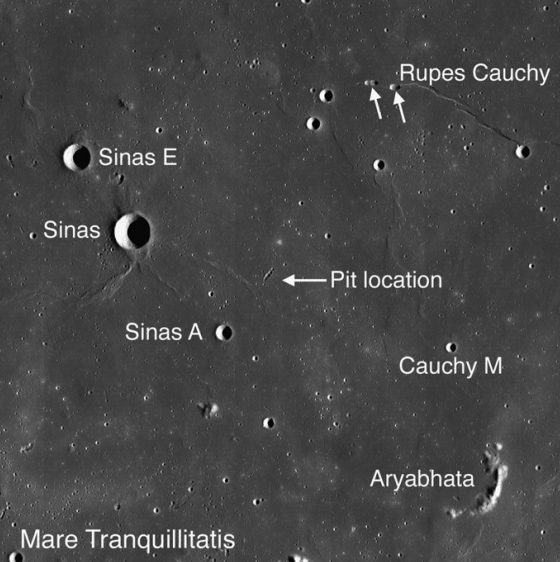
\includegraphics[width=0.9\linewidth]{Lunar_Pit_layers_2pic_location.png}
        \caption{Location of the Mare Tranquillitatis pit, captured by \textbf{LRO WAC}. Figure adapted from \cite{sublunear-lava}.}
        \label{fig:image2}
    \end{subfigure}
\end{figure}

\subsection{Discovery and Recognition}
The identification of lunar pits was delayed until the advent of advanced lunar missions, as these features are relatively small and difficult to observe using Earth-based telescopes \cite{lunar-pit-distribution}. Early evidence emerged from SELENE and LRO data, which revealed steep-walled pits with distinct overhangs and evidence of hollow subsurface structures. For instance, the Mare Tranquillitatis pit has been confirmed to connect to a subsurface void, tens of meters long, using radar and gravitational techniques, transforming pits from geological curiosities to priority targets for lunar exploration \cite{Carrer2024, GRAIL, radar-observations-lava-tubes}.

The Mare Tranquillitatis pit, in particular, has been the focus of radar and imaging studies that confirmed its connection to a subsurface cave conduit. These findings not only demonstrate the scientific value of pits for studying lunar geology but also highlight their potential for human exploration. Advanced thermal modeling, such as that performed using Diviner data, shows that the interior of pits remains thermally stable compared to the extreme surface environment, reinforcing their suitability as habitats or resource storage sites \cite{newer-thermal, lunar-pits-entrances-to-caves, thermal-lunar-pits}.

As technology advances, the exploration of lunar pits continues to evolve. With 3D thermal models, radar imaging, and gravitational studies, these features are increasingly seen as critical to understanding the Moon’s history and unlocking future possibilities for sustained human presence on its surface \cite{newer-thermal, radar-observations-lava-tubes, grails-gradients-mariushills}.
\newpage

\graphicspath{{img/ch2}}

\section{Lunar Pit Geological Characteristics}

\subsection{Morphological Characteristics}

Lunar pits exhibit distinct morphological features that provide critical insights into their geological origins and evolution. They typically feature a funnel-shaped upper region leading into near-vertical walls, often ending in flat or concave floors \cite{new-wagner}. The sharp transition between the sloping entrance and vertical walls suggests sudden roof collapse above a subsurface void, rather than gradual erosion processes \cite{lunar-pits-numerical-modelling, lunar-pits-entrances-to-caves}.

\begin{figure}[h!]
    \centering
    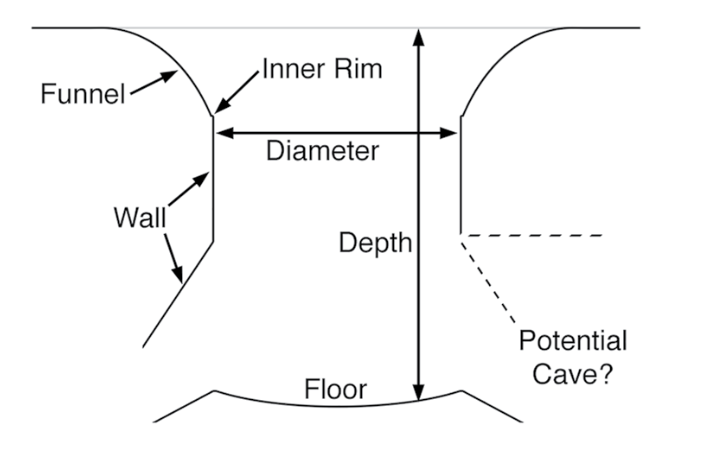
\includegraphics[width=0.5\linewidth]{lunar_pit_schema.png}
    \caption{A simplified schematic of a generic lunar pit cross-section showing key morphological features (adapted from \cite{new-wagner}).}
    \label{fig:lunar-pit-schema}
\end{figure}

High-resolution images from the Lunar Reconnaissance Orbiter (LRO) Narrow Angle Camera (NAC) have revealed significant details, such as layering within pit walls. These layers, likely corresponding to successive volcanic flow events, provide a geological record of ancient lunar volcanism \cite{new-wagner}. Observations of overhangs within pits, particularly at Marius Hills and Mare Tranquillitatis, suggest access to extensive subsurface voids, often interpreted as collapsed lava tubes \cite{lunar-pits-entrances-to-caves, Carrer2024}. These voids could be tens of meters in length and offer compelling targets for future exploration \cite{lava-tube-observations}.

The base of lunar pits typically contains accumulations of boulders and regolith. Some pits exhibit concave floors, contributing significantly to their depth and distinguishing them from traditional impact craters, which feature raised rims and ejecta blankets \cite{new-wagner}.

\begin{figure}[H]
    \centering
    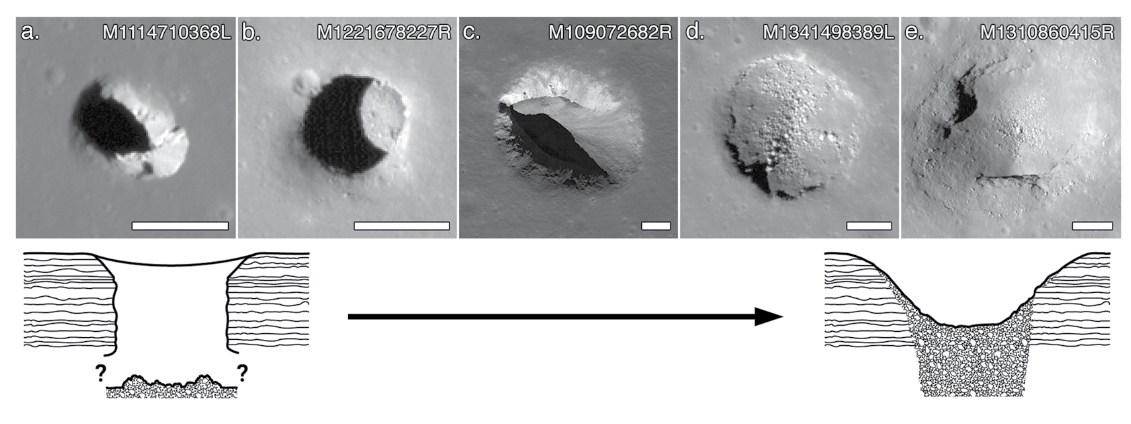
\includegraphics[width=0.85\linewidth]{closed_and_open_cavities.png}
    \caption{Progression of lunar pit degradation, illustrating gradual erosion and regolith deposition over time. Figure shows different lunar pits in various stages of erosion (adapted from \cite{new-wagner}).}
    \label{fig:lunar-pit-degradation}
\end{figure}

Over geological timescales, lunar pits degrade due to micrometeoroid impacts, thermal cycling, and seismic activity. These processes erode walls and rims, depositing debris at the base. Some pits, such as those in Mare Tranquillitatis and Marius Hills, show varying states of preservation, with sharp walls in younger features and smoother, infilled floors in older examples \cite{lunar-pit-distribution}. The degradation process operates independently of the surrounding terrain age, suggesting pits evolve gradually over hundreds of millions of years \cite{new-wagner, lunar-pits-numerical-modelling}.

\subsection{Geographical Distribution and Formation Mechanisms}

Lunar pits are distributed across three primary geological settings: mare basalts, impact melt deposits, and highland terrain. These pits provide a unique window into the Moon's geological evolution and are formed by distinct mechanisms based on their location and context \cite{lunar-pit-distribution, lunar-pits-numerical-modelling}.

\begin{figure}[H]
    \centering
    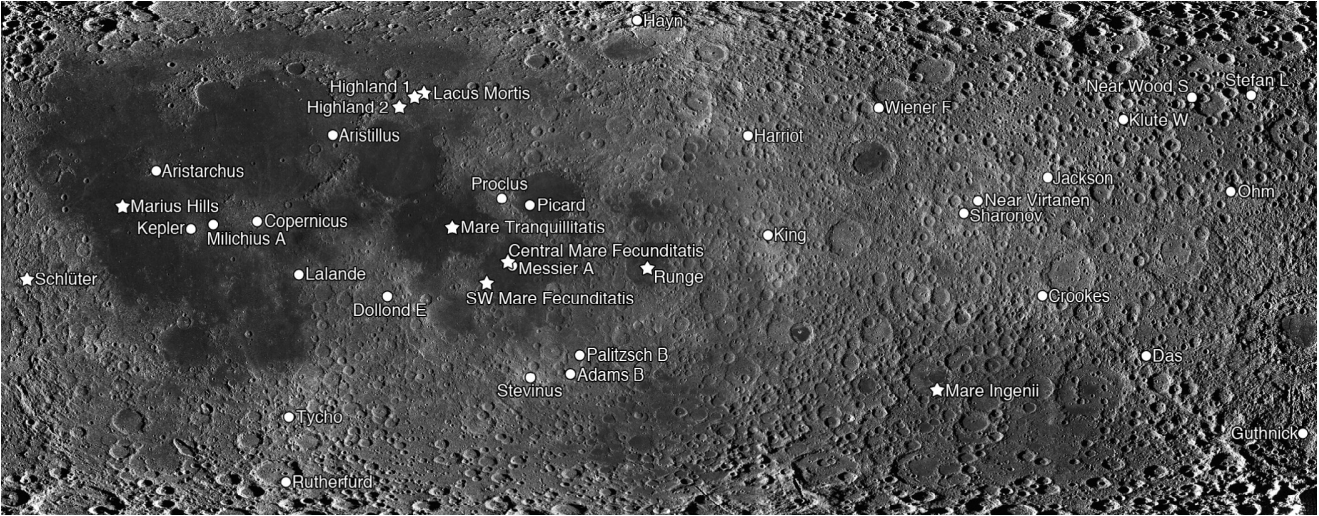
\includegraphics[width=0.76\linewidth]{map-lunar-pits-rough.png}
    \caption{Map of lunar pits: eight in mare basalts, two in highlands (stars), and 29 in impact melt deposits (dots). Figure adapted from \cite{lunar-pit-distribution}.}
    \label{fig:map-lunar-pits}
\end{figure}

\paragraph{Mare Basalts} Pits in mare regions, such as Marius Hills and Mare Tranquillitatis, are primarily linked to volcanic activity. These pits likely form due to the collapse of lava tube roofs, where thinning overlying material becomes unstable and collapses into subsurface voids \cite{lunar-pits-entrances-to-caves}. Such pits are often found near sinuous rilles, which are remnants of ancient volcanic flow channels, further indicating their volcanic origin. For instance, radar and imaging data from the Mare Tranquillitatis pit revealed an extensive subsurface void consistent with a collapsed lava tube \cite{Carrer2024, lava-tube-observations} (see \ref{fig:image1}). These features not only indicate ancient volcanic activity but also provide potential access to well-preserved lava tube interiors.

\begin{figure}[H]
    \centering
    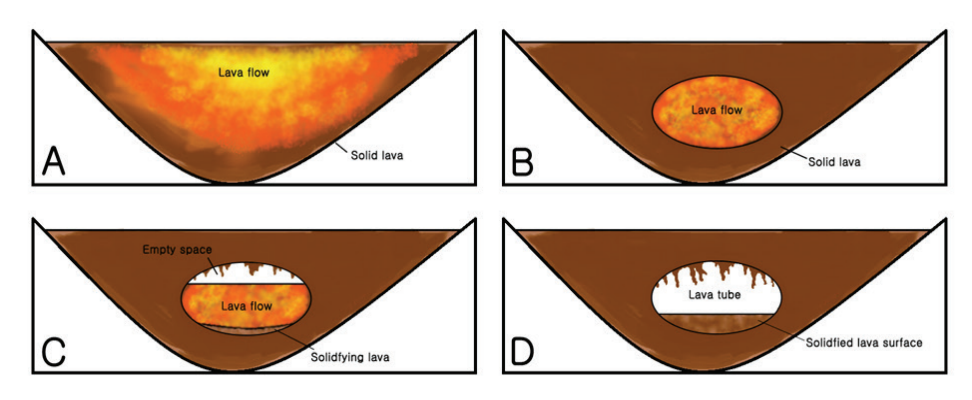
\includegraphics[width=0.7\linewidth]{lava_tube_formation_schema.png}
    \caption{Stages of lunar lava tube formation, illustrating crust solidification, lava drainage, and resulting voids (adapted from \cite{lunar-pits-entrances-to-caves}).}
    \label{fig:lava-tube-formation-schema}
\end{figure}

\paragraph{Impact Melt Deposits} Pits found within younger impact craters, such as Tycho and Copernicus, form due to a combination of impact-generated processes. High-energy impacts fracture and compress the lunar crust while generating immense heat that melts surface and subsurface material. This molten impact melt redistributes across the crater floor, forming pools of rapidly cooling material. During solidification, thermal contraction creates extensive cracks and fractures \cite{new-wagner}. Simultaneously, void spaces can develop where molten material drains or collapses into pre-existing subsurface cavities. Over time, localized collapses along these fractures or voids form impact melt pits \cite{lunar-pits-numerical-modelling, lunar-pit-distribution}. Unlike volcanic pits, these features are typically more circular in shape, lack overhangs, and show no association with lava flows.

\begin{figure}[H]
    \centering
    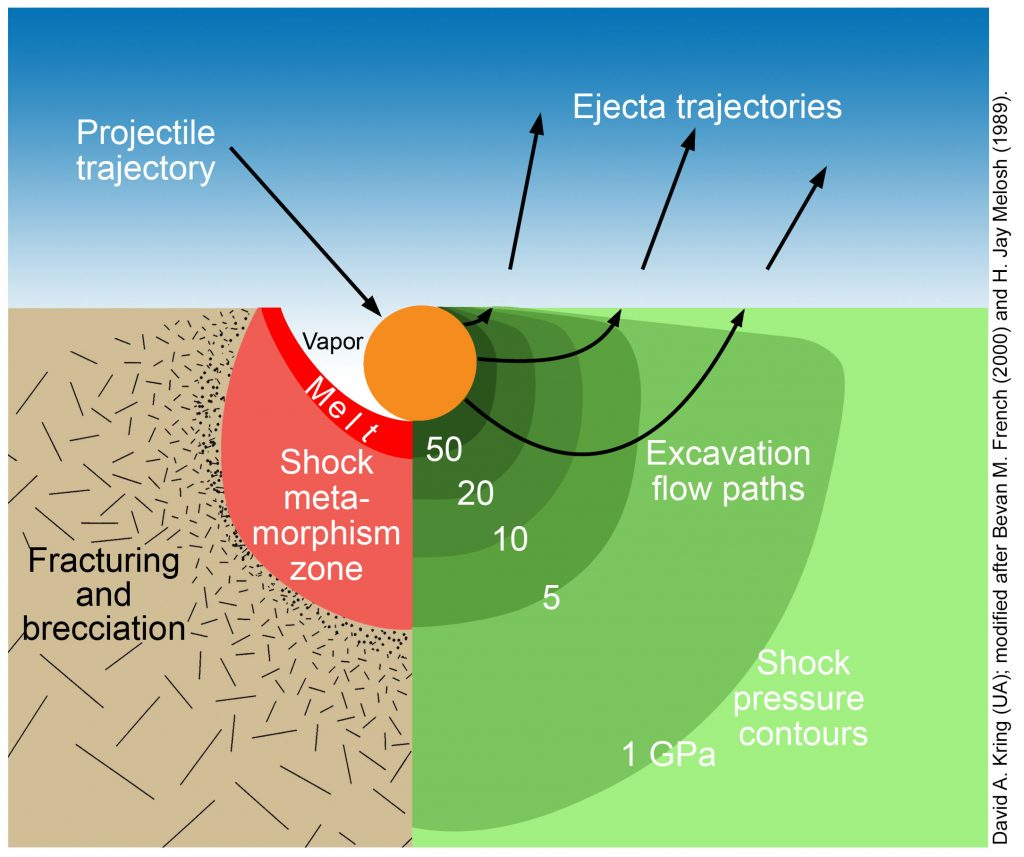
\includegraphics[width=0.42\linewidth]{Impact-Shock-Pressures-and-Their-Effects-1024x857.jpg}
    \caption{Impact dynamics illustrating pressure zones, molten material, formation of cracks, contributing to pit formation in impact melt deposits (adapted from     \cite{clrn-impact-melt}).}
    \label{fig:impact-melt}
\end{figure}

\paragraph{Highland Terrain} Highland pits are rare and thought to result from tectonic stress and extensional faulting. These pits typically form near large-scale graben systems or faulted regions, where crustal stress generates fractures in the lunar surface. Over time, localized collapse along these fault zones forms pits with sharp, near-vertical walls \cite{new-wagner}. Examples include the Lacus Mortis pit and pits in the Rima Hyginus region, which are situated along prominent grabens. Unlike mare pits, highland pits lack volcanic features or associations with lava tubes, making their tectonic origins more evident \cite{lunar-pit-distribution}.

\begin{figure}[H]
    \centering
    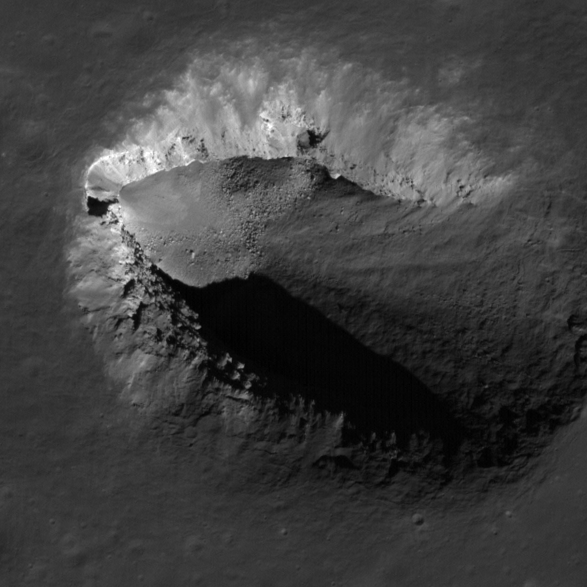
\includegraphics[width=0.33\linewidth]{lunar-pit-highland.png}
    \caption{Lunar Reconnaissance Orbiter Camera footage of Lacus Mortis Pit. Image adapted from: \url{https://www.lroc.asu.edu/atlases/pits}.}
    \label{fig:highland-lunar-pit}
\end{figure}

\paragraph{Impact-Induced Skylights}form when small meteoroid impacts trigger the collapse of thin crusts overlying intact subsurface voids, such as lava tubes. Unlike traditional impact craters, these skylights lack ejecta blankets and raised rims because the impact energy is localized and primarily directed toward destabilizing the roof material \cite{lunar-pits-numerical-modelling}.

For example, the Marius Hills pit provides a compelling case: numerical models suggest that a meteoroid impact on a 26-meter-thick roof caused its collapse, forming a skylight approximately 40 meters in diameter. The underlying void remained intact, but the shock wave and resulting fractures weakened the overlying material enough to cause it to cave in \cite{clrn-impact-melt}.

\begin{figure}[H]
    \centering
    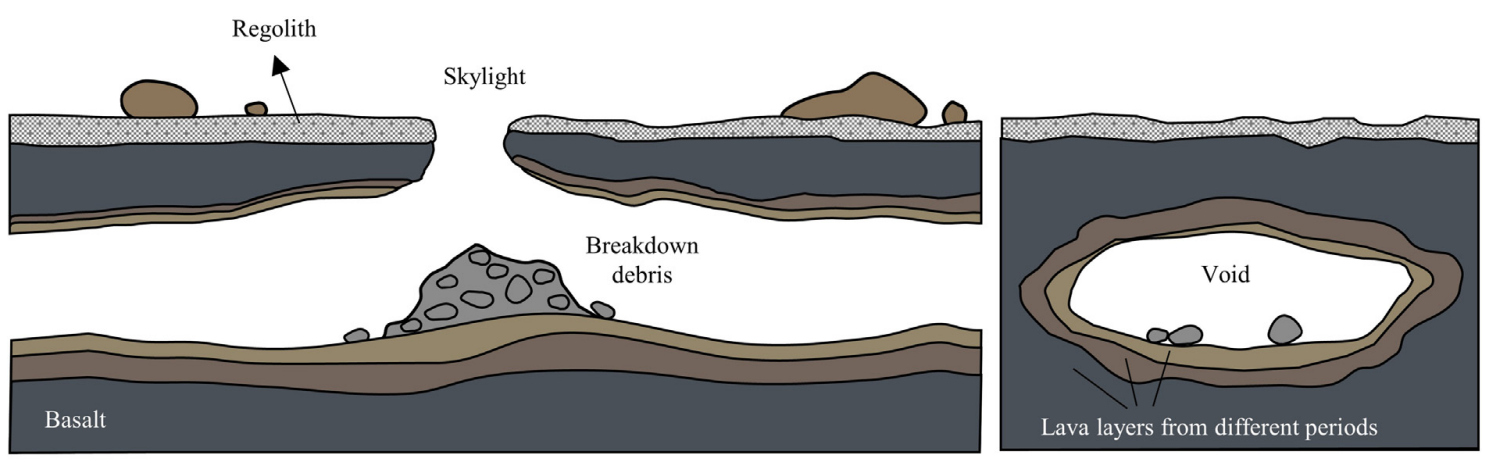
\includegraphics[width=0.99\linewidth]{lunar-pit-in-lava-tube.png}
    \caption{Cross section of a lunar tube with collapsed skylight (adapted from    \cite{bases-feng}).}
    \label{fig:impact-induced-skylight}
\end{figure}


\graphicspath{{img/ch3}}

\section{Thermal Characteristics}

\subsection{Thermal Stability and Anomalies}

The thermal environment within lunar pits provides a stark contrast to the extreme temperature fluctuations of the lunar surface. Data collected from the Diviner Lunar Radiometer Experiment reveal that the interior of pits maintains remarkably stable temperatures, ranging from 250 to 290 K in permanently shadowed regions, even during the lunar night \cite{thermal-lunar-pits}. This contrasts with the lunar surface, where temperatures vary dramatically between $\sim$100 K at night and $\sim$400 K in direct sunlight due to the Moon’s lack of atmosphere \cite{newer-thermal}.

\begin{figure}[H]
    \centering
    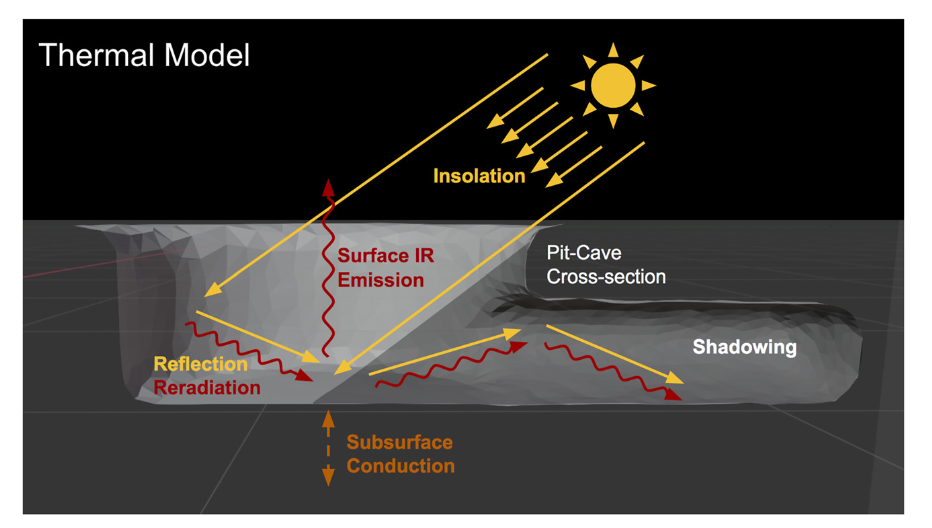
\includegraphics[width=0.6\linewidth]{lunar-pit-thermal-model.png}
    \caption{Schematic representation of heat transfer in lunar pits, illustrating shadowing, infrared emission, and subsurface conduction \cite{thermal-lunar-pits, newer-thermal}.}
    \label{fig:lunar-pit-thermal-model}
\end{figure}

The thermal stability results from the geometry of the pits, with overhanging walls and limited sky exposure blocking direct solar radiation and mitigating radiative heat loss during the lunar night. This configuration creates natural “blackbody cavities,” as modeled by Horvath et al. \cite{thermal-lunar-pits}, leading to effective absorption and internal redistribution of heat. For instance, pits such as those in Mare Tranquillitatis and Mare Ingenii have floors that remain up to 100 K warmer than their surroundings at night \cite{thermal-lunar-pits, newer-thermal, nesnas2019}.

The location of lunar pits relative to the equator or poles significantly impacts their thermal behavior. Pits closer to the equator, such as those in Mare Tranquillitatis, experience more extreme daytime temperature peaks due to higher levels of direct sunlight. In contrast, pits located closer to the poles maintain more stable temperatures, making thermal management less challenging. However, polar pits receive less sunlight, which reduces the availability of solar energy for power generation and may require hybrid energy systems to support exploration missions \cite{thermal-lunar-pits, newer-thermal}.

\begin{figure}[H]
    \centering
    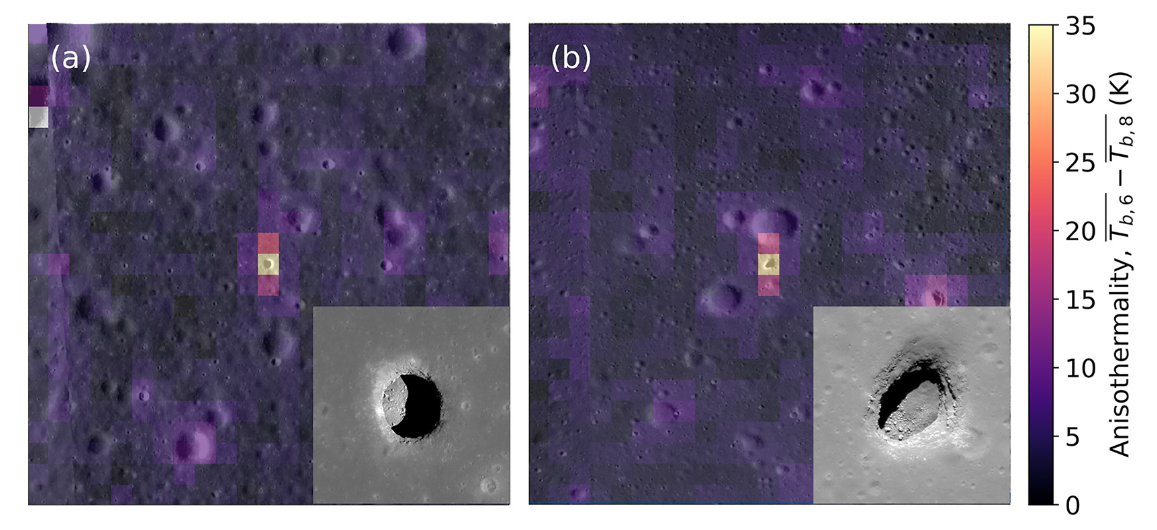
\includegraphics[width=0.7\linewidth]{lunar-pits-temperature-LROC.png}
    \caption{Temperature maps of Mare Tranquillitatis (a) and Mare Ingenii pits (b) measured by Diviner. Insets show NAC images for reference. Warm anomalies appear in pit interiors compared to surrounding surfaces \cite{thermal-lunar-pits}.}
    \label{fig:lunar-pits-temperatures-LROC}
\end{figure}

\subsection{Thermal Dynamics and Material Effects}

The thermal behavior of pit floors and walls depends strongly on their material composition. Regolith-dominated floors exhibit higher diurnal temperature variations due to their insulating properties, leading to pronounced daytime peaks and nighttime minima. In contrast, rock-dominated surfaces show smaller variations, as their higher thermal conductivity allows for more efficient heat transfer and equilibrium \cite{thermal-lunar-pits, newer-thermal}.

\begin{figure}[H]
    \centering
    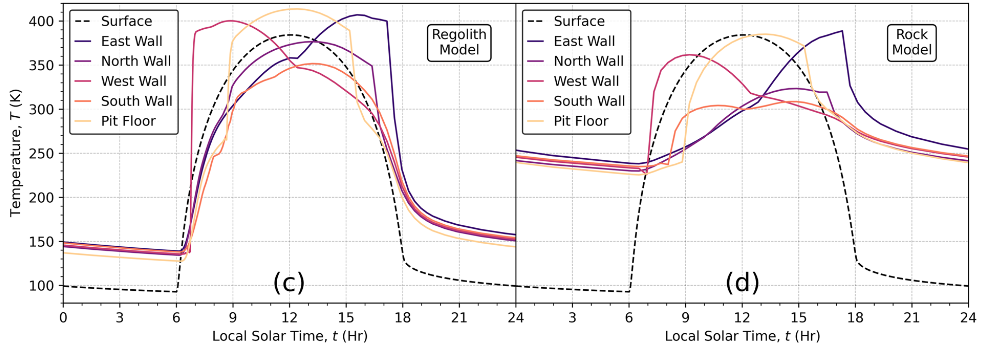
\includegraphics[width=0.9\linewidth]{lunar-pit-regolith-vs-stone-thermal.png}
    \caption{Simulated temperature profiles for lunar pits assuming regolith (c) and solid rock (d) floors. Rock surfaces show smaller diurnal variations due to higher thermal conductivity, while regolith exhibits greater fluctuations \cite{thermal-lunar-pits}.}
    \label{fig:regolith-vs-stone-thermal}
\end{figure}

The thermal behavior of lunar pits is strongly influenced by the nature of their floors. Pits with rocky floors maintain temperatures closer to equilibrium, as rock surfaces efficiently distribute absorbed heat, making them attractive for potential habitation and exploration. In contrast, regolith-covered floors retain heat near their openings and exhibit extreme thermal gradients. These gradients, resulting from the low thermal conductivity of lunar regolith, pose challenges for thermal management, especially during extended missions \cite{thermal-lunar-pits, newer-thermal}.

Numerical simulations show that rocky pit walls experience lower peak daytime temperatures and more gradual temperature variations compared to regolith surfaces, which insulate heat and cause significant temperature extremes. These properties highlight the need for tailored exploration strategies depending on the pit's material composition \cite{thermal-lunar-pits, lunar-pits-numerical-modelling}.

\begin{figure}[H]
    \centering
    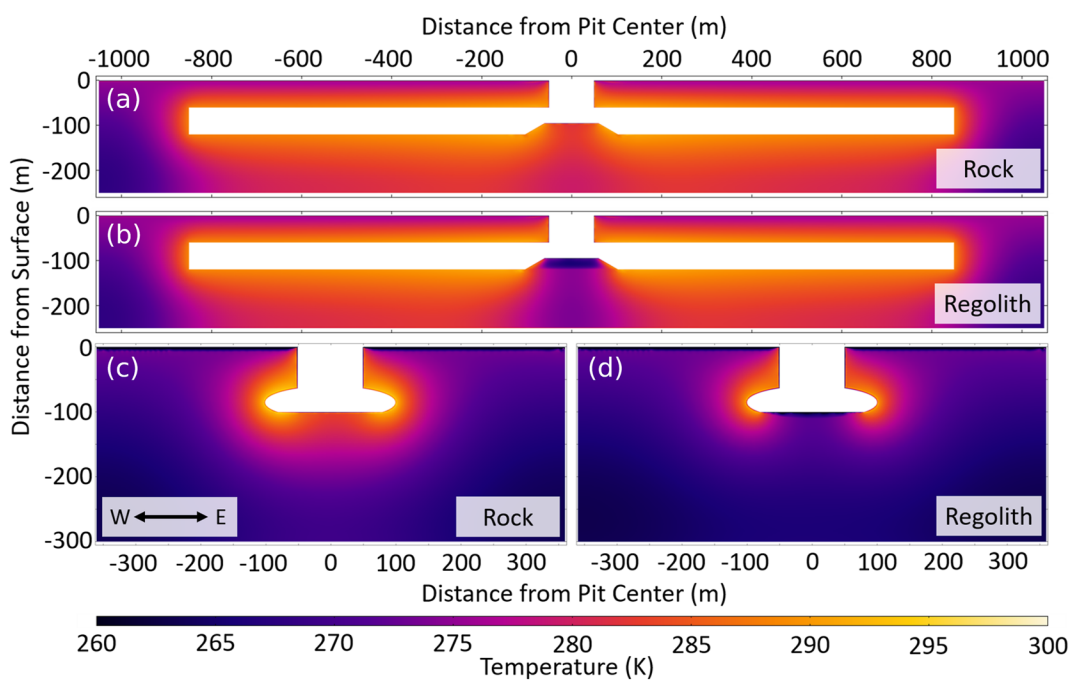
\includegraphics[width=0.8\linewidth]{thermal-simulation-lunar-pits-2d-regolith-rock.png}
    \caption{Equilibrium temperature distributions for rock (a, c) and regolith (b, d) surfaces in lunar pits and caves. Rock surfaces exhibit cooler and more uniform internal temperatures due to higher thermal conductivity, while regolith retains heat closer to the opening, leading to pronounced thermal gradients. Adapted from \cite{thermal-lunar-pits}.}
    \label{fig:lunar-pit-equilibrium-temps}
\end{figure}


\subsection{Volatile Stability and Cold Traps}

While lunar pits have been proposed as potential cold traps for volatiles like water ice, recent studies show that their enclosed geometry raises internal temperatures through multiple-scattered infrared radiation (see Fig. \ref{fig:lunar-pit-thermal-model}). This reduces their efficiency compared to traditional craters \cite{newer-thermal}. Nevertheless, specific conditions—such as pits shadowed by exterior topography or connected to deeper caves—could still support volatile accumulation \cite{thermal-lunar-pits, lunar-pits-numerical-modelling}.

Latitude affects volatile retention within pits. Pits closer to the poles experience lower maximum temperatures and are less likely to lose volatiles to sublimation compared to equatorial pits. However, the geometry of polar pits can still lead to elevated internal temperatures compared to permanently shadowed regions (PSRs), limiting their efficiency as long-term volatile storage sites \cite{newer-thermal, lunar-pits-numerical-modelling}.

Wilcoski et al. \cite{newer-thermal} demonstrate that while volatile loss rates in pits are higher than in PSRs, certain configurations—such as pits with deeper caves or extended shadowed regions—may still allow for temporary volatile preservation. These findings suggest that lunar pits could serve as short-term repositories for accessible volatiles during exploration missions.


\graphicspath{{img/ch4}}

\section{Evidence of Cavities Beneath Lunar Pits}

Evidence for subsurface cavities beneath lunar pits is derived from morphological observations, geophysical gravity anomalies, radar sounder reflections, and thermal data. These findings point to large, interconnected voids beneath regions such as \textbf{Marius Hills} and \textbf{Mare Tranquillitatis}, supporting their interpretation as remnants of ancient lava tubes and key features of lunar geological evolution.

\subsection{Morphological Evidence}

Overhanging walls and roof collapses in lunar pits strongly suggest access points to larger subsurface voids, such as intact lava tubes (see Fig. \ref{fig:image1}). High-resolution imagery from the Lunar Reconnaissance Orbiter (LROC) has revealed alignments between these pits and sinuous rilles—ancient lava flow channels associated with underground tubes \citep{lunar-pits-entrances-to-caves, grails-gradients-mariushills}. The Marius Hills region, in particular, shows clear morphological correlations with known volcanic features, as seen in Figure~\ref{fig:marius-hills-collapse}.

\textbf{Collapse Chains and Pit Alignments:} Linear sequences of pits, known as collapse chains, further support the hypothesis of underlying cavities. These chains represent the progressive collapse of lava tube roofs, forming surface depressions that trace the subsurface voids. This is particularly evident in Marius Hills, where pit alignments correlate with surface rilles and lava tubes observed on Earth \citep{new-wagner, cavities-selene-lavatubes}.

\begin{figure}[H]
    \centering
    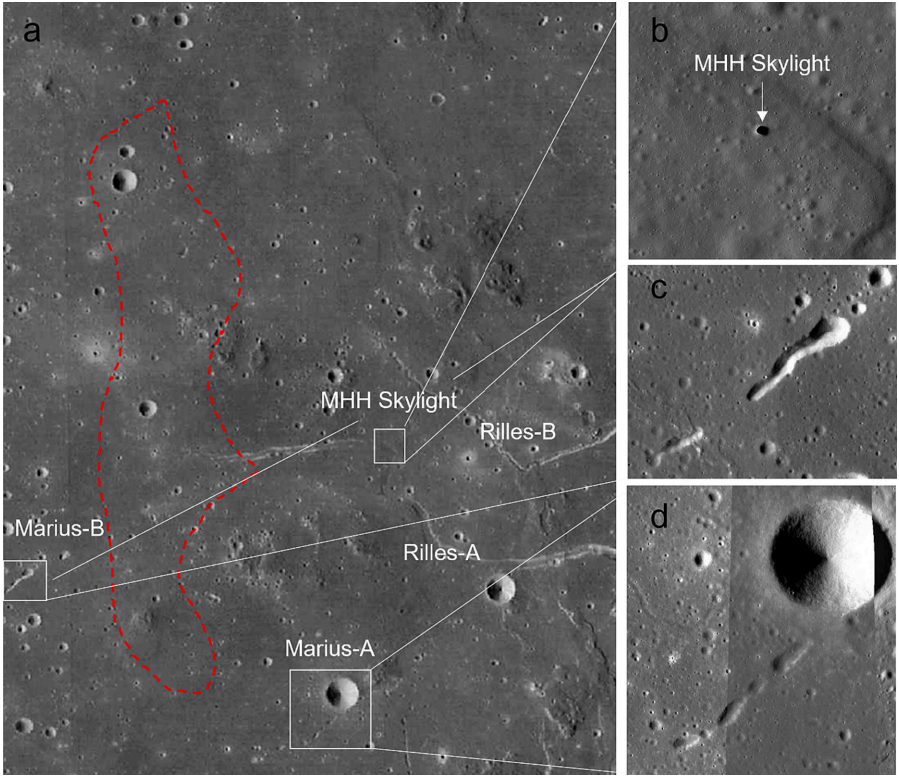
\includegraphics[width=0.5\linewidth]{marius_hills_collapse.png}
    \caption{LROC WAC image of the Marius Hills region, showing collapse chains, sinuous rilles, and skylights. The red dashed line marks the approximate path of the subsurface lava tube. 
    \textbf{(a)} Overview of the Marius Hills region with localized collapse chains and skylights. 
    \textbf{(b)} Close-up of the Marius Hills Hole (MHH). 
    \textbf{(c)} Marius-B collapse chain. 
    \textbf{(d)} Marius-A collapse chain. 
    Adapted from \citet{grails-gradients-mariushills}.}
    \label{fig:marius-hills-collapse}
\end{figure}

\subsection{Geophysical Evidence}

\textbf{Gravity Anomalies from GRAIL:} Subsurface cavities induce detectable gravitational anomalies due to mass deficits in hollow regions. Data from the \textbf{Gravity Recovery and Interior Laboratory (GRAIL)} mission has revealed mass deficits beneath several pit locations. For example, in Marius Hills, Bouguer gravity gradients identified a hollow structure approximately 60 km long and 9 km wide at a depth of 600 m \citep{grails-gradients-mariushills}. These anomalies align closely with pit locations and other volcanic features.

\begin{figure}[H]
    \centering
    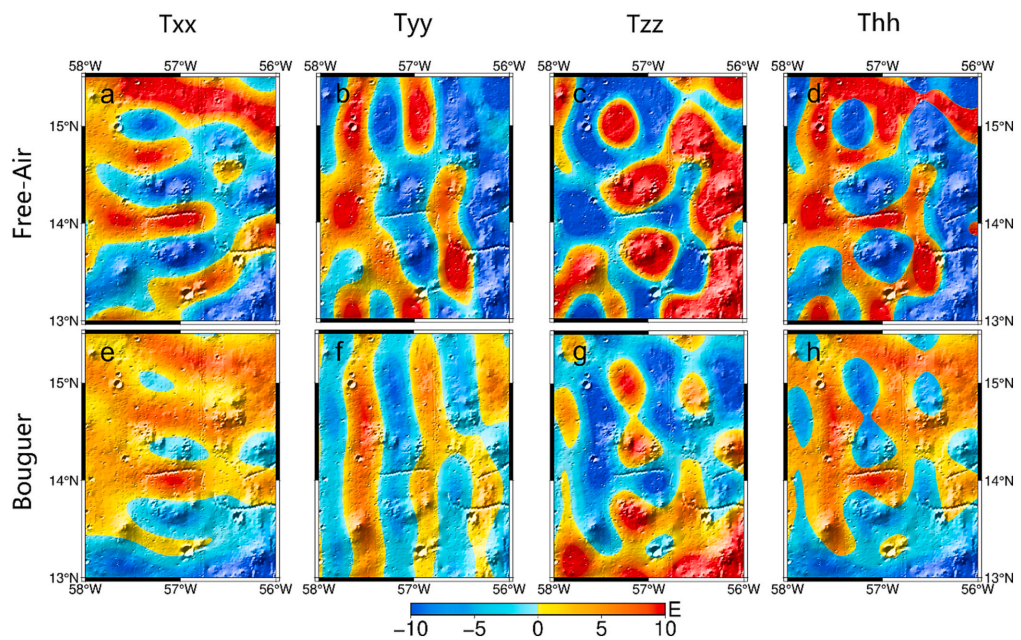
\includegraphics[width=0.85\linewidth]{grail-images-grabity.png}
    \caption{Gravitational anomalies in the Marius Hills region detected by GRAIL. Bouguer gravity gradients reveal mass deficits (blue), indicative of subsurface voids such as intact lava tubes. Adapted from \citet{grails-gradients-mariushills}.}
    \label{fig:marius-hills-gravity}
\end{figure}

\subsection{Radar Evidence from SELENE and Mini-RF}

\textbf{Radar Echoes from SELENE (Kaguya):} Radar sounders like the Lunar Radar Sounder (LRS) onboard SELENE have been instrumental in confirming subsurface cavities. Double-echo patterns—secondary radar reflections—indicate voids beneath the lunar surface. At Mare Tranquillitatis, LRS data suggest a subsurface cavity extending several kilometers \cite{cavities-selene-lavatubes}.

\begin{figure}[H]
    \centering
    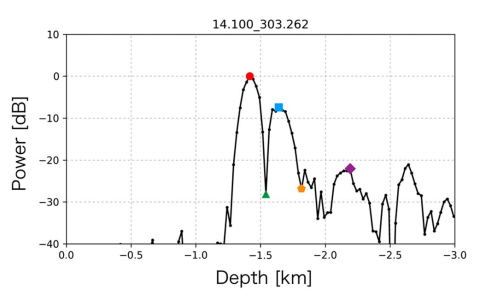
\includegraphics[width=0.35\linewidth]{selene-doublebump.png}
    \caption{SELENE LRS radar echoes showing a characteristic double-echo pattern indicative of a subsurface void. The first peak represents the surface reflection, while the second peak corresponds to the void floor. Adapted from \cite{cavities-selene-lavatubes}.}
    \label{fig:radar-echoes}
\end{figure}

\textbf{Mini-RF Contributions:} Using Mini-RF data, Carrer et al. (2024) identified radar reflections beyond the walls of Mare Tranquillitatis Pit. These reflections are consistent with a lava tube connected to the pit. Combined with gravitational and morphological data, this strengthens the hypothesis of intact subsurface voids \cite{Carrer2024}.

\begin{figure}[H]
    \centering
    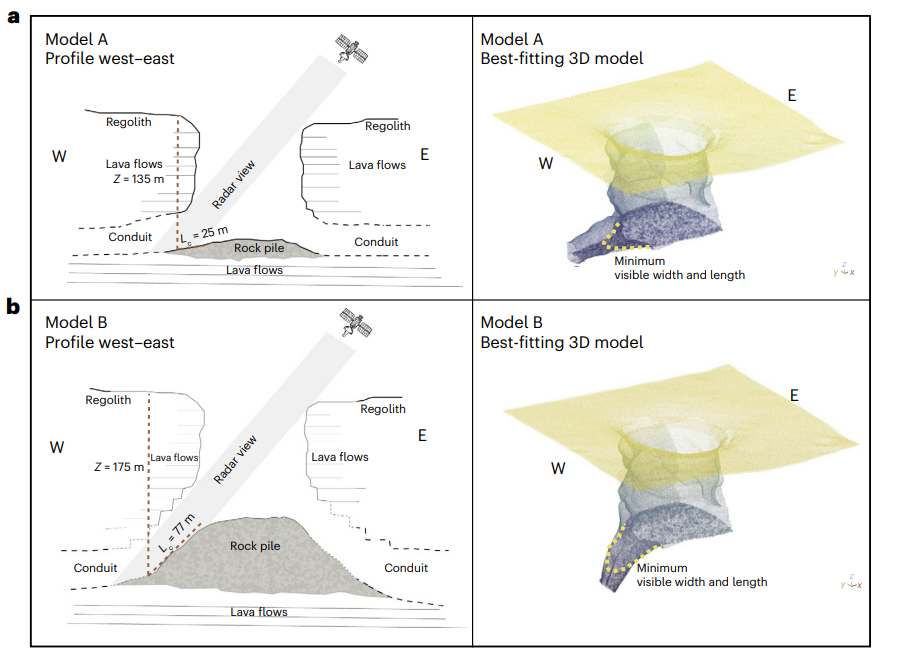
\includegraphics[width=0.85\linewidth]{carrer-renders.png}
    \caption{Reconstructed Mare Tranquillitatis Pit (MTP) cave conduit based on inversion of Mini-RF radar data. \textbf{(a)} Model A with a conduit of approximately 135 m width and a low floor slope. \textbf{(b)} Model B with a conduit approximately 175 m wide and steeper floor slopes. The 3D models show the surface (yellow), subsurface lava flows (blue), and inferred lava tube conduit (gray). Adapted from \cite{Carrer2024}.}
    \label{fig:mtp-cave-conduit}
\end{figure}

\subsection{Thermal Observations as Indirect Evidence}

Thermal data also suggest subsurface cavities beneath pits. The Diviner Lunar Radiometer Experiment has shown that the interiors of pits maintain stable temperatures, supporting the idea of thermally buffered environments consistent with underground voids. For example, temperatures within the Mare Tranquillitatis pit remain near -25°C throughout the lunar night, suggesting limited thermal exposure due to cavity geometry \cite{thermal-lunar-pits, newer-thermal}.

This stability aligns with the blackbody cavity effect, where limited exposure to sunlight and the insulating properties of surrounding rock create stable conditions. Such environments could provide ideal conditions for exploration and resource utilization.

\graphicspath{{img/ch5}}

\section{Upcoming Missions}

Lunar pits have become a focal point for future exploration due to their potential for subsurface access, resource extraction, and habitat construction. Robotic missions will pave the way for human exploration by mapping pit interiors, assessing geological stability, and searching for subsurface cavities.

\subsection{Robotic Missions to Lunar Pits}

Robotic exploration is essential for investigating the geometry, stratigraphy, and resource potential of lunar pits. Several upcoming missions aim to explore the interiors of pits, providing key data to support future human missions.

\subsubsection{NASA's Daedalus Rover}

The **Daedalus rover** is a spherical, autonomous robotic explorer designed to map pit interiors. Using **LIDAR, panoramic cameras, and environmental sensors**, Daedalus can roll along the pit floor, collect data, and generate **3D models of walls and cavities**. It descends into pits using a tethered system, which ensures continuous power and data transmission. The mission aims to confirm the presence of voids and assess subsurface stability \cite{thermal-lunar-pits, newer-thermal}.

\subsubsection{ESA's Tethered Sphere Robot}

The **European Space Agency (ESA)** is developing a similar **tethered exploration system**, which allows the robot to descend into pits while remaining connected to a surface lander. Unlike NASA's free-roaming Daedalus, ESA's version focuses on stable descent and precise mapping of pit interiors. The tether provides **constant power and data relay**, reducing operational risks. This mission will study pit wall composition, stability, and signs of subsurface voids \cite{thermal-lunar-pits}.

\subsubsection{Lunar Reconnaissance Orbiter (LRO) Follow-up Surveys}

While LRO has already provided detailed images and radar scans of pits, future follow-up surveys will focus on **reprocessing LRO datasets with machine learning algorithms**. These methods will improve the detection of thermal anomalies, overhangs, and cavity signatures. **Mini-RF radar** will play a key role in scanning subsurface features, with particular focus on pits like **Mare Tranquillitatis** and **Marius Hills**, where previous radar reflections hinted at potential subsurface cavities \cite{Carrer2024, new-wagner}.

\subsubsection{Private and Commercial Missions}

Private space companies like **Astrobotic** and **ispace** are also planning robotic missions to survey lunar pits, leveraging technologies such as **ground-penetrating radar (GPR)**, LIDAR, and thermal imaging. These missions aim to characterize pit interiors and assess their viability for **resource extraction and human settlement**. By mapping key pits near potential Artemis landing sites, private missions could support future human exploration goals \cite{jsanders-isru}.

---

\subsection{Human Exploration of Lunar Pits}

Future **Artemis missions** aim to explore and assess the habitability of lunar pits. While Artemis III will focus on the lunar south pole, subsequent missions (e.g., Artemis V) are expected to target sites like **Mare Tranquillitatis** and **Marius Hills**, which show strong evidence of subsurface voids and stable overhangs \cite{new-wagner, Carrer2024}.

\subsubsection{Human Descent Technologies}

Exploring the vertical walls of pits presents unique technical challenges. Proposed methods for human descent include:
\begin{itemize}
    \item **Tethered descent systems**: Astronauts could rappel into pits using robotic winches or climbing gear. 
    \item **Legged robotic scouts**: Autonomous robots or climbers could precede astronauts, identifying safe routes for descent.
    \item **Aerial drones**: Drones could provide high-resolution maps of pit interiors and locate points of interest for human exploration \cite{thermal-lunar-pits, newer-thermal}.
\end{itemize}

---

\subsection{Scientific Objectives for Upcoming Missions}

Future missions will address several key scientific objectives. Lunar pits offer direct access to subsurface geology, potential resources, and stable environments for future exploration.

\subsubsection{Access to Stratigraphy}

Pit walls expose the Moon's **stratigraphy**, revealing stacked layers of ancient lava flows. By analyzing these layers, scientists can reconstruct the **volcanic history of the Moon** and investigate how lava tube systems evolved. Stratigraphic differences at pits like **Mare Tranquillitatis** and **Marius Hills** suggest regional variations in volcanic activity \cite{new-wagner}.

\subsubsection{Detection of Subsurface Cavities}

A major goal of upcoming missions is the detection of **subsurface cavities** beneath pit floors. Cavity detection will rely on **ground-penetrating radar (GPR)**, **gravitational anomaly analysis**, and **Mini-RF radar scans**. Observations of radar reflections at **Mare Tranquillitatis** have already revealed possible subsurface voids \cite{Carrer2024}. By confirming the presence of accessible voids, missions could identify potential sites for resource extraction and habitation.

\subsubsection{Search for Volatiles and Water Ice}

Pits located near **permanently shadowed regions (PSRs)** may act as **traps for water ice and volatiles**. The interior geometry of pits, particularly those with overhanging structures, creates localized cold environments where volatiles could accumulate. Missions will use **infrared spectrometers** and radar to detect water ice, which is essential for **In-Situ Resource Utilization (ISRU)**. Extracted water could be converted into hydrogen and oxygen, serving as **rocket fuel and life support** for human missions \cite{jsanders-isru}.

---

\subsection{Summary of Key Missions and Technologies}

\begin{itemize}
    \item **NASA's Daedalus Rover** — Spherical robotic explorer for 3D mapping and void detection \cite{thermal-lunar-pits}.
    \item **ESA's Tethered Sphere Robot** — Tethered robotic explorer focused on stability and power efficiency \cite{thermal-lunar-pits}.
    \item **Artemis V Missions** — Human-led missions to survey and explore pits using tethered descent and climbers \cite{thermal-lunar-pits}.
    \item **LRO Follow-up Surveys** — Advanced radar and machine learning analysis to detect subsurface cavities \cite{Carrer2024, new-wagner}.
    \item **Private Missions** — Robotic scouts from companies like Astrobotic and ispace to explore potential Artemis landing sites \cite{jsanders-isru}.
\end{itemize}

\graphicspath{{img/ch6}}

\section{Human Habitation in Lunar Pits and Lava Tubes}

Lunar pits and lava tubes offer a transformative solution for sustainable human habitation on the Moon. These geological formations provide natural protection from the harsh lunar environment and a unique opportunity for long-term exploration and settlement.

\subsection{Advantages of Lunar Pits and Lava Tubes for Habitation}

Lunar pits and lava tubes present several inherent benefits:
\begin{itemize}
    \item \textbf{Radiation Shielding:} The thick layers of regolith above these features reduce exposure to harmful cosmic rays and solar radiation, providing a safer environment for habitation \cite{thermal-lunar-pits}.
    \item \textbf{Thermal Stability:} Unlike the surface, which experiences extreme temperature fluctuations, the interiors of pits and tubes maintain near-constant temperatures around -20$^\circ$C, conducive to equipment and human activities \cite{thermal-lunar-pits}.
    \item \textbf{Micrometeoroid Protection:} Subsurface voids naturally shield against micrometeoroid impacts, ensuring safety for infrastructure and inhabitants \cite{lunar-pits-entrances-to-caves}.
    \item \textbf{Volatile Retention:} Pits and tubes potentially trap volatiles such as water ice in their shadowed interiors, vital for life support and in-situ resource utilization (ISRU) \cite{newer-thermal}.
\end{itemize}

\subsection{Habitation Concepts}

\textbf{Modular Inflatable Habitats:}
Inflatable habitats provide a lightweight and flexible solution for pressurized living spaces. These structures can be deployed within the protective confines of lava tubes, minimizing exposure to external hazards. Prefabrication on Earth further reduces complexities during deployment \cite{bases-feng}.

\textbf{3D-Printed Infrastructure:}
Advanced 3D printing technologies enable the construction of robust infrastructure using lunar regolith. Applications include structural walls, radiation shields, and support systems, reducing dependency on Earth-supplied materials \cite{jsanders-isru}. This approach also enhances sustainability by leveraging local resources.

\begin{figure}[H]
    \centering
    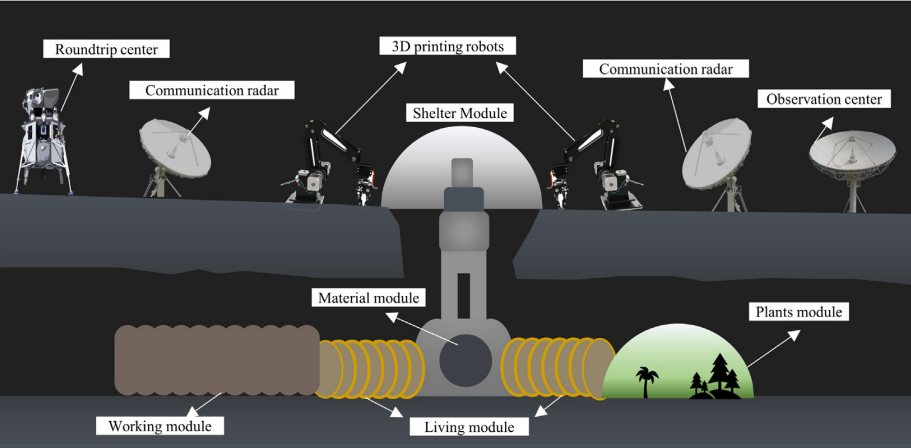
\includegraphics[width=0.8\linewidth]{simple-base-schema.png}
    \caption{Conceptual design of a lunar base within a pit. Overhangs provide natural shielding, while modular inflatable habitats create pressurized living spaces. Adapted from \cite{bases-feng}.}
    \label{fig:lunar-habitat}
\end{figure}

\textbf{Layered Habitat Modules:}
The verticality of lava tubes enables multi-tiered habitat designs, integrating living spaces, laboratories, and storage areas. This approach optimizes spatial utilization while maintaining functionality and safety \cite{sublunear-lava}.

\textbf{Hydroponic Farming Modules:}
The controlled environments within lava tubes are ideal for hydroponic farming, allowing astronauts to cultivate food and sustain life independently of Earth. The lack of surface hazards further supports efficient agricultural operations \cite{bases-feng}.

\subsection{Resource Utilization and Sustainability}

\textbf{Water Extraction:}
Water ice in permanently shadowed regions near pits can be harvested for drinking water, oxygen generation, and fuel production. Technologies such as the extraction of oxygen from regolith complement this effort, enabling closed-loop resource cycles \cite{jsanders-isru}.

\textbf{Energy Solutions:}
Solar panels installed on the surface near pits, combined with tethered power systems, can deliver consistent energy to subsurface habitats. Small modular reactors may complement these systems during lunar nights, ensuring uninterrupted power supply \cite{lro}.

\textbf{Material Processing:}
Using regolith for construction materials through sintering or chemical reduction not only supports structural needs but also enhances mission sustainability by reducing launch payloads \cite{jsanders-isru}.

\subsection{Challenges and Future Directions}

While promising, the habitation of lunar pits and lava tubes presents several challenges:
\begin{itemize}
    \item \textbf{Access and Exploration:} Advanced robotics such as tethered rovers (e.g., Daedalus) and jumping robots are critical for safely exploring and assessing the structural stability of these features \cite{esa-daedalus}.
    \item \textbf{Structural Assessment:} Determining the geological stability of lava tubes and their resistance to collapse is essential for planning long-term habitation \cite{sublunear-lava}.
    \item \textbf{Human Factors:} Prolonged habitation requires addressing psychological and physiological challenges associated with living in isolated, confined environments.
\end{itemize}


\graphicspath{{img/ch7}}

\section{Conclusion}
Lunar pits have transitioned from geological curiosities to critical components of lunar exploration. They offer a direct link to the Moon's subsurface, revealing stratigraphic records and enabling in-depth volcanic analysis. Beyond scientific inquiry, pits hold the potential to become cornerstones of human exploration, serving as natural habitats, storage areas, and ISRU hubs. 

By providing thermal stability, radiation shielding, and access to essential resources, pits could support sustainable lunar missions. Robotic and human expeditions will convert theoretical concepts into practical applications, solidifying pits as vital elements of the lunar exploration architecture. Their study and exploitation could define the future of humanity's presence on the Moon, shaping how we explore and inhabit extraterrestrial environments.


\bibliographystyle{plainnat}
\bibliography{references}

\end{document}
